\documentclass{article}
\usepackage[utf8]{inputenc}
\usepackage[a4paper,top=3cm,bottom=2cm,left=3cm,
right=3cm,marginparwidth=1.75cm]{geometry}
\usepackage{amsmath} %for \text inside math mode and matrices
\usepackage{graphicx}
\usepackage{subcaption}
\usepackage{mdframed}

\title{ECE 2300 - Lab 2 Report}
\author{Stephen Chin and Aryaa Pai}
\date{Due: February 20}

\graphicspath{{./figs/}}


\begin{document}
\maketitle

\section{Introduction}

The overall goal of this lab was to successfully decode a 4-bit
input to an output number display on a seven section decoder. The lab
was split into two sections, both involving breadboarding inputs to
create a successful display. The first part allowed all inputs to be
sent through a CMOS CD4511B 7-segment decoder, allowing us to test our
initial breadboard setup, battery, and inputs. The second part allowed
us to wire the decoders for inputs $c$, $e$, and $g$ using only NAND
gates and inverters.

The materials allowed to us in this lab consisted of a breadboard, two
72LS00 2-input NAND gate chips, one 72LS04 NOT gate, one 72LS10
3-input NAND gate, one 72LS20 4-input NAND gate, one CMOS CD4511B 7-
segment decoder, one 74LS241 buffer, a resistor array, a 7-segment
input display, along with a battery and a voltage regulator.

During our time in the lab, we were able to complete our design,
achieving a fully functioning 7 segment display output on all digits 0
to 9. Although difficult to implement, we were able to take our
pre-designed circuit and wire it correctly on the breadboard.


\section{Design}

The design of our logic circuit was based on the process of logic
minimization through the use of Karnaugh maps. In order to create a
minimized logic function for each segment of the 7-segment display, we
created Karnaught maps for each of the outputs based on a truth table
created from looking at the desired outputs. By our design
specification, we were able to consider all inputs 10-15 to be ''don't
cares'', simplifying our logic expressions.


\begin{figure}[h!]
  \begin{mdframed}
  \centering
  \begin{subfigure}[b]{0.3\linewidth}
    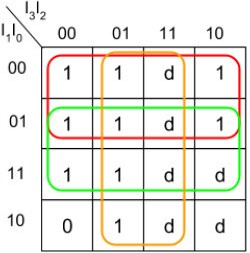
\includegraphics[width=\linewidth]{c_kmap.jpg}
    \caption{K-map for c.}
  \end{subfigure}
  \begin{subfigure}[b]{0.3\linewidth}
    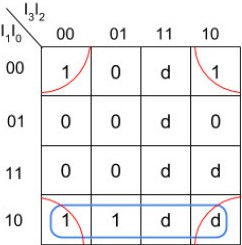
\includegraphics[width=\linewidth]{e_kmap.jpg}
    \caption{K-map for e.}
  \end{subfigure}
  \begin{subfigure}[b]{0.3\linewidth}
    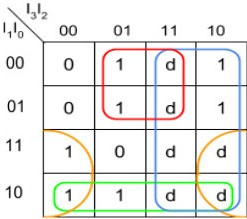
\includegraphics[width=\linewidth]{g_kmap.jpg}
    \caption{K-map for g.}
  \end{subfigure}
  \end{mdframed}
  \caption{The karnaugh maps for the segments c, e, and g.}
\end{figure}

The karnaugh maps provided the boolean logic for each of the three
segments of the display. From there, we were able to write out boolean
logic expressions and implement them using the CMOS chips allowed in
the lab.


\section{Implementation}




\section{Testing}

For part 1 of the lab, we tested the 7-segment decoder and display
by sending each valid 4-bit input into the decoder. If the display
shows the valid output for the 4-bit input, then we know that our
circuit is properly wired. For part one, we did not run into any major
problems involving wiring, and we were able to complete it without any
major setbacks.

For part 2, we tested our decoder and digital logic in essentially the
same way as in part 1, by running the valid inputs through our
circuits. For this part, we ran into multiple problems involving our
wiring. We had a short in our circuit due to some wiring issues of
inputs being wired to other inputs. We miswired one our decoder
outputs to the incorrect segment on the decoder.

The major difficulty of debugging our wiring problems was correctly
identifying the problem from the breadboard and our outputs. The
symptoms of each problem were either a single section of the display
not working, or that the display would not work entirely. These
symptoms did not give us enough information to identify the problem,
as they could have been seen as a result of many other problems
instead. For example, when we had a short in our circuit, our first
idea was to check the power rails on the sides of the breadboard, then
to check the battery, and then to check the power going to each of the
chips. All of the problems that we checked for could have been
diagnosed by the same symptoms, making it incredibly hard to properly
debug the circuits we were making.

However, we were able to mitigate some of the frustrations of
debugging through other means when wiring our breadboard. First of
all, we color-coded our input wires so that we could tell at a glance
where a wire was intended to be from/going to. Though there were many
connections that we had to check, the color coding we used helped us
visualize our intended circuit. Another tactic we used was to create
many different power and ground rails, allowing us to wire power and
ground neatly, eliminating unnecessary wire crossover. Although it did
not rid our circuit of bugs, what we did helped us visualize what our
problems were.


\section{Conclusion}

For this lab, we wired a 7-segment display partially through a
decoder, and partially manually. For the decoded outputs, we simply
passed our inputs through the decoder chip and resistor array to the
correct terminals on the 7-segment display. For our wired decoder on
outputs $c$, $e$, and $g$, we used NAND gate chips to implement the
logic function specified for the outputs.

What we learned in this lab was how to generate minimized boolean
expressions from Karnaugh maps, how to understand design
specifications to create ''don't cares'' in our maps, and the process
of wiring a complicated circuit on a breadboard.


\section{Work Distribution}

During the lab, both of us brought in our finished wiring designs from
the output boolean expressions. While we were wiring the circuit, we
ended up splitting the different parts of the wiring between the two
of us, as one person would finish wiring the rails and chip
connections as the other routed the inputs and outputs to their
positions on the breadboard as per our design. For this lab report, we
also split the work. While one person worked on the design and
implementation sections of the report, the other worked on the
testing, introduction, and conclusion.



\end{document}

